\documentclass[11pt,a4paper,openany]{report}
\usepackage[T1]{fontenc}
\usepackage[utf8]{inputenc}
\usepackage{lmodern}
\usepackage{microtype}
\usepackage{amsmath,amssymb,amsthm,mathtools,bm}
\usepackage{booktabs,array,longtable,tabularx}
\usepackage{xcolor}
\usepackage[margin=22mm,headheight=23pt]{geometry}
\usepackage{enumitem}
\usepackage{fancyhdr}
\usepackage{fancyvrb}
\usepackage{graphicx}
\usepackage{url}
\usepackage{xurl}
\usepackage{hyperref}
\definecolor{finblue}{HTML}{1F5A99}
\definecolor{fingreen}{HTML}{19733A}
\definecolor{finorange}{HTML}{D55E00}
\definecolor{finred}{HTML}{A61B1B}
\definecolor{finviolet}{HTML}{6A3D9A}
\definecolor{fingray}{HTML}{4D4D4D}
\hypersetup{
  unicode=true,
  colorlinks=true,
  linkcolor=finblue,
  citecolor=fingreen,
  urlcolor=finblue,
  pdftitle={FIN Programs 255--266: Operator Memory Measures, Identifiability, Current Tomography and Adaptive-Analogy Falsification},
  pdfauthor={Krzysztof Żuchowski},
  pdfsubject={Executed FIN research Programs 255--266 and recommended Programs 267--280},
  pdfkeywords={FIN, operator-valued Stieltjes functions, Schur complement, memory kernels, process information, current tomography, identifiability, reservoir computing}
}
\pagestyle{fancy}
\fancyhf{}
\fancyhead[L]{\small Programy FIN 255--266}
\fancyhead[R]{\small Release 10.24}
\fancyfoot[C]{\thepage}
\setlength{\parindent}{0pt}
\setlength{\parskip}{0.55em}
\setlist{nosep,leftmargin=2em}
\setcounter{tocdepth}{2}
\setcounter{secnumdepth}{3}
\emergencystretch=3em
\newcommand{\one}{\bm 1}
\newcommand{\C}{\mathbb C}
\newcommand{\R}{\mathbb R}
\newcommand{\Z}{\mathbb Z}
\newcommand{\statusProven}{\textcolor{fingreen}{[Proven]}}
\newcommand{\statusStrong}{\textcolor{finblue}{[Strong evidence]}}
\newcommand{\statusModerate}{\textcolor{finviolet}{[Moderate evidence]}}
\newcommand{\statusWeak}{\textcolor{fingray}{[Weak evidence]}}
\newcommand{\statusSpeculative}{\textcolor{finorange}{[Speculative]}}
\newcommand{\statusRefuted}{\textcolor{finred}{[Refuted]}}
\begin{document}
\hypersetup{pageanchor=false}
\begin{titlepage}
\centering
\vspace*{11mm}
{\Large\bfseries FIN --- Release 10.24\par}
\vspace{10mm}
{\Huge\bfseries Programy badawcze 255--266\par}
\vspace{5mm}
{\LARGE\bfseries Miary operatorowe pamięci, identyfikowalność,\\
tomografia prądów i falsyfikacja analogii adaptacyjnych\par}
\vspace{16mm}
{\Large Krzysztof \.Zuchowski\par}
\vspace{2mm}
{\normalsize Independent Researcher --- Fractal Information Theory Project\par}
\vspace{2mm}
{\normalsize ORCID: \href{https://orcid.org/0009-0002-0909-3613}{0009-0002-0909-3613}\par}
\vspace{9mm}
{\large 28 lipca 2026\par}
\vfill
\begin{minipage}{0.9\textwidth}
\small
\textbf{Centralny wynik.}
Dla każdego nietrywialnego kontekstu strict \(Z_{12}\):
\[
\Sigma_E(z)=\int_{(0,\infty)}\frac{d\mathsf M_E(\mu)}{z+\mu},
\qquad d\mathsf M_E(\mu)\succeq0.
\]
Pamięć określa minimalną klasę realizacji wejście--wyjście, a nie unikalny
sektor mikroskopowy.

\medskip
\textbf{Granica.}
Raport nie eksportuje selektora, skali fizycznej, pełnego mostu
legacy--strict, prawa adaptacji ani walidacji laboratoryjnej.

\medskip
\textbf{Repozytorium.}
\url{https://github.com/hyconiek/Fractal-Nadsoliton-Theory}

\textbf{Licencja.} CC BY 4.0.
\end{minipage}
\vfill
\end{titlepage}
\hypersetup{pageanchor=true}
\pagenumbering{roman}
\tableofcontents
\clearpage
\pagenumbering{arabic}

\chapter*{Konwencja pewności}
\addcontentsline{toc}{chapter}{Konwencja pewności}

\begin{itemize}
\item 
\textbf{\statusProven{}} --- wynik wynika z jawnego dowodu skończenie wymiarowego albo ścisłej to\.zsamości; obliczenie numeryczne jest tylko certyfikatem.

\item 
\textbf{\statusStrong{}} --- deterministyczny, odtwarzalny audyt syntetyczny z zamro\.zonym modelem i progiem.

\item 
\textbf{\statusModerate{}} --- stabilny wynik w zadanej klasie, lecz zale\.zny od dodatkowej definicji lub równowa\.zności.

\item 
\textbf{\statusSpeculative{}} --- skonstruowany program lub obiekt bez wystarczającego dowodu.

\item 
\textbf{\statusRefuted{}} --- jawny kontrprzykład albo no-go w zadanej klasie.

\end{itemize}

Status matematyczny nie jest statusem fizycznym. W szczególności \statusProven{} nie oznacza, \.ze operator został zrealizowany przez przyrodę.

\chapter{1. Executive summary}

Wykonano wszystkie programy 255--266. Najwa\.zniejsze wyniki są następujące.

\begin{enumerate}
\item 
Dla ka\.zdego z \(2^{12}-2=4094\) nietrywialnych kontekstów \(E\subset Z_{12}\) samoenergia

\[
   \Sigma_E(z)=A_{EH}(zI+A_{HH})^{-1}A_{HE}
   \]

jest transformatą dodatniej skończonej miary operatorowej i jest całkowicie monotoniczna. \textbf{\statusProven{}}

\item 
Deklarowany sześciowymiarowy sektor ukryty w podziale even/\allowbreak{}odd ma tylko pięć wymiarów widzialnych przez \(\Sigma_E\). Jeden tryb jest dokładnie niewidoczny. Dodanie dowolnych dalszych rozsprzę\.zonych trybów nie zmienia samoenergii. \textbf{\statusProven{}}

\item 
Konteksty i redukcje Schura tworzą kontrawariantną kategorię. Zło\.zenie redukcji jest łączne; maksymalny residual w 20 000 łańcuchach wynosi \(6.66\times10^{-16}\). Nie udowodniono aksjomatów snopa. \textbf{\statusProven{}}

\item 
Chiralna podatność pamięci ma zamknięty wzór:

\[
   \Xi_E
   =B'RB^\ast+BRB'^\ast-BRC'RB^\ast,
   \qquad R=(zI+C)^{-1}.
   \]

Jest nieparzysta pod inwersją i spełnia jawne ograniczenie normy. Pozostaje odbiornikiem zadanego skrętu, nie źródłem orientacji. \textbf{\statusProven{}}

\item 
Naiwny dynamiczny RG oparty wyłącznie na ścisłym zmniejszaniu kontekstu \(12\to6\to3\to1\) nie ma nietrywialnego fixed pointu ani cyklu w kategorii, której obiekt zachowuje wymiar. Potrzebna jest nowa, jawna size-restoring equivalence. \textbf{\statusProven{}}

\item 
Zbudowano wieloczasowy bilans rozró\.znialności:

\[
   D_{\rm in}
   =
   \mathcal L_{\rm env}
   +D_{\rm record}
   +D_{\rm conditional}.
   \]

Bilans teleskopuje z residualem zero, ale nie jest jeszcze termodynamiką. \textbf{\statusProven{}}

\item 
Zamro\.zona przed testem mapa mostu usuwająca tylko amplitudę \(\alpha_{\rm geo}\) nie przenosi legacy do dodatniej klasy generatorów strict. Legacy ma \(\lambda_{\min}=-7.7101\), a jego blok ukryty generuje biegun na dodatniej osi \(z=5.8248\). Jest to no-go tylko dla amplitude-only completion. \textbf{\statusProven{}}

\item 
Syntetyczny protokół fingerprint-first/\allowbreak{}calibration-second przechodzi 300/\allowbreak{}300 prób przy 50 000 zliczeń na przygotowanie, lecz nie zastępuje zewnętrznego pakietu P241 i nie uruchamia P242. \textbf{\statusStrong{}}

\item 
Sam vertex POVM nie identyfikuje prądów. Skonstruowano dwa dodatnie stany \(\rho\) i \(\rho^\ast\) o identycznych populacjach i przeciwnych prądach. Potrzebne są obserwable interferometryczne. \textbf{\statusProven{}}

\item 
Atlas false positives pokazuje, \.ze dodatniość Stieltjesa i składanie Schura są ogólne dla dodatnich Laplasjanów, a nie swoiste dla FIN. Najbardziej swoisty jest fingerprint widmowy. \textbf{\statusProven{}} dla zamro\.zonych zespołów.

\item 
Bez niezale\.znego zegara \((cA,t)\) i \((A,ct)\) są dokładnie nierozró\.znialne. Pamięć aparatu wymaga danych wieloczasowych, a zmiana kształtu generatora jest widoczna w fingerprint. \textbf{\statusProven{}}

\item 
Benchmark biologiczno-cybernetyczny daje wynik negatywny dla przewagi FIN: pojemność pamięci wynosi \(4.0601\) i jest ni\.zsza ni\.z we wszystkich 120 kontrolach, natomiast powrót po zaburzeniu jest najwolniejszy. FIN jest odró\.znialnym, silnie wygładzającym rezerwuarem, ale nie wykazano przewagi obliczeniowej ani biologicznej. \textbf{\statusStrong{}}

\end{enumerate}

\begin{figure}[htbp]
\centering
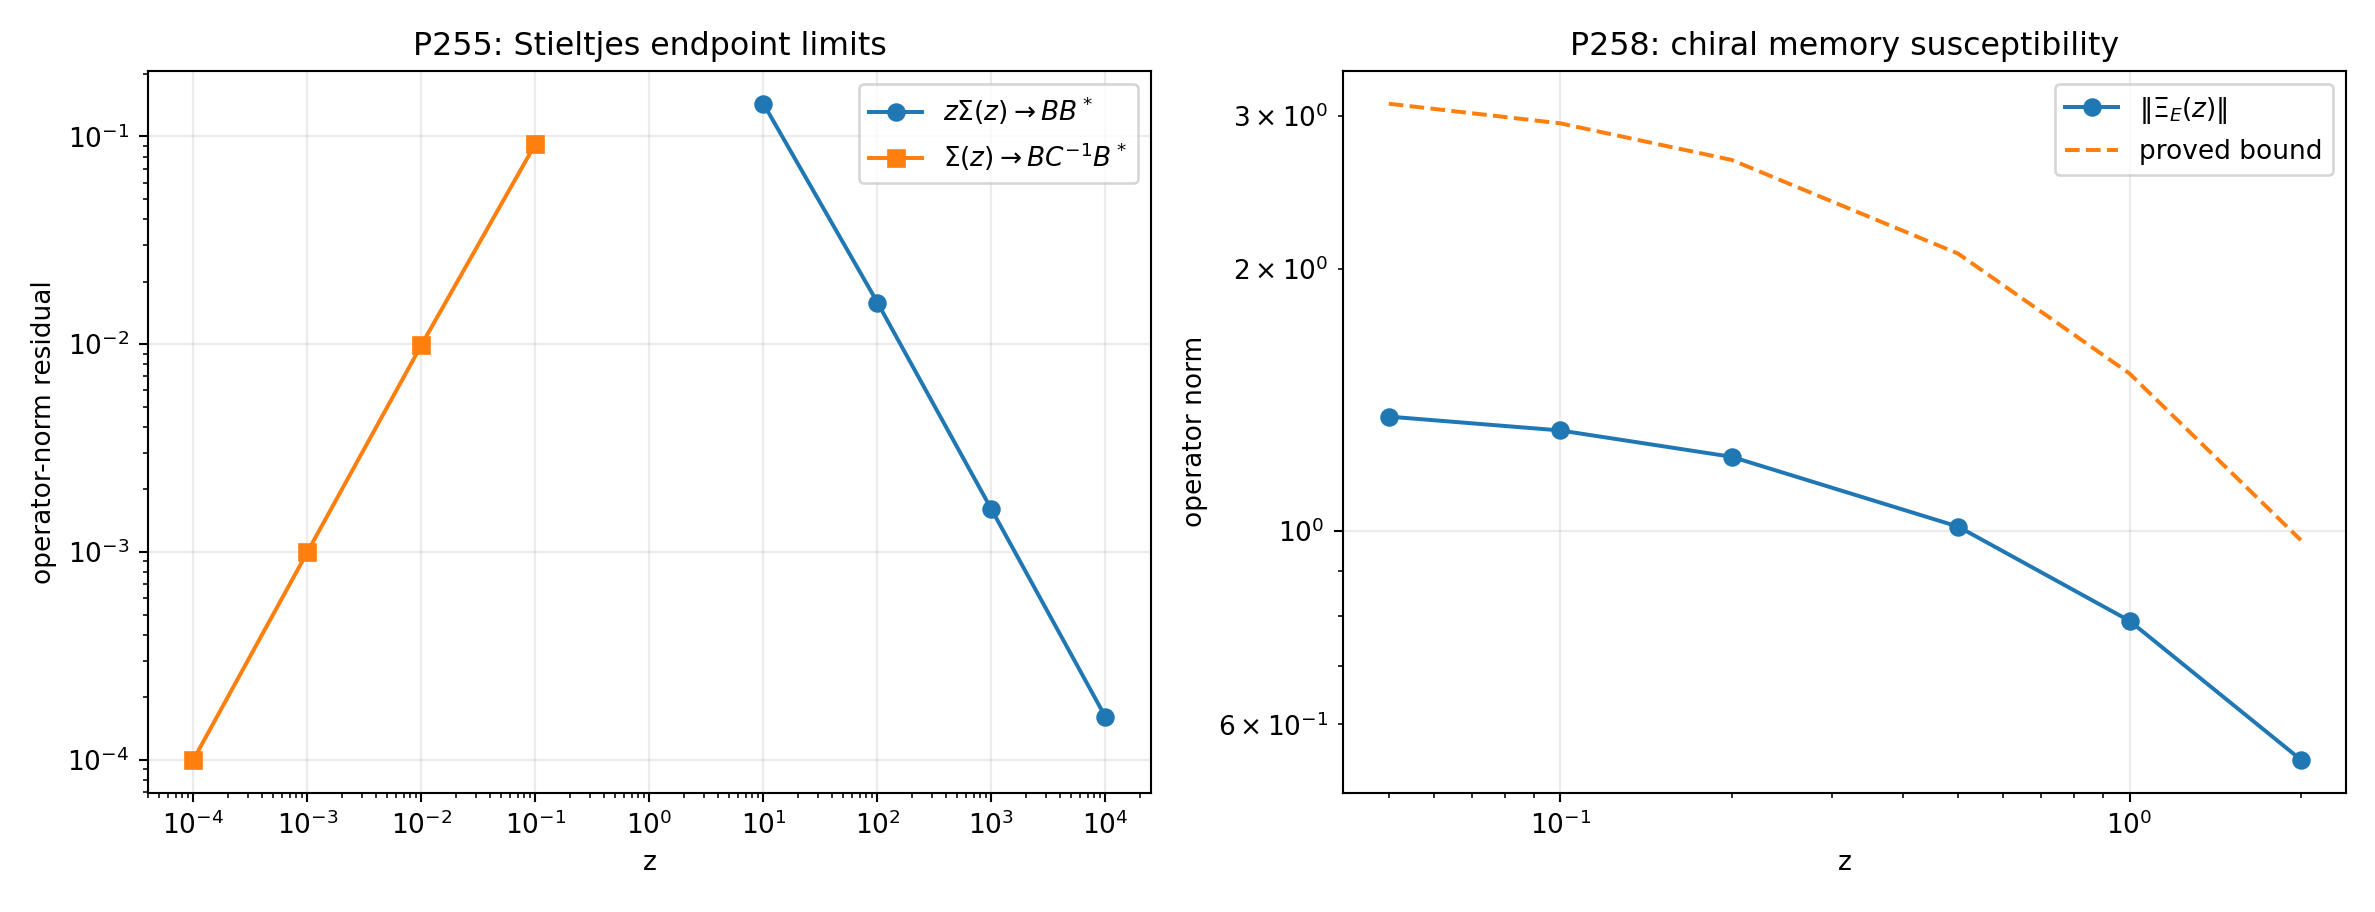
\includegraphics[width=0.97\textwidth]{FIN_Programs_255_266_Figures/p255_p258_stieltjes_chiral.png}
\caption{Granice funkcji Stieltjesa oraz norma chiralnej podatności pamięci wraz z udowodnionym ograniczeniem.}
\end{figure}

\chapter{2. Zamro\.zony rdzeń i zakres}

Pracujemy z rzeczywistym symetrycznym operatorem strict:

\[
W_{xy}=K_{\rm strict}(d(x,y)),\qquad
A=\operatorname{diag}(W\mathbf 1)-W.
\]

Dla:

\[
K_{\rm strict}(d)
=
\frac{\cos(0.18575\,d+0.16250)}{1+d^{1.8}},
\qquad d=1,\ldots,6,
\]

otrzymujemy:

\[
A=A^\ast,\qquad A\mathbf 1=0,\qquad A\succeq0.
\]

Podział \(V=E\sqcup H\) oznacza jedynie operacyjny podział dostępnych i ukrytych stopni swobody nadsolitona. Nie wprowadza warstwy informacyjnej "pod" nadsolitonem.

W obliczeniach:

\begin{itemize}
\item 
u\.zyto deterministycznego ziarna 20260729;

\item 
nie u\.zyto danych laboratoryjnych;

\item 
nie dostrajano progów po wynikach;

\item 
w P261 zamro\.zono tylko jeden atom mostu;

\item 
zachowano oddzielenie legacy i strict;

\item 
nie u\.zyto Firecrawl.

\end{itemize}

\chapter{3. Macierz wyników}

\begin{center}
\begingroup\small
\setlength{\tabcolsep}{2.5pt}
\renewcommand{\arraystretch}{1.16}
\begin{longtable}{@{}p{0.117\textwidth}p{0.362\textwidth}p{0.100\textwidth}p{0.280\textwidth}@{}}
\toprule
\textbf{Program} & \textbf{Wynik} & \textbf{Status} & \textbf{Najwa\.zniejsza granica} \\
\midrule
\endhead
P255 & dodatnia miara operatorowa dla 4094 kontekstów & \statusProven{} & nie dowodzi fizycznego środowiska \\
P256 & minimalny wymiar ukryty \(=5\), a nie 6 & \statusProven{} & mikroskopowa realizacja nieunikalna \\
P257 & kontrawariantna kategoria Schura & \statusProven{} & brak twierdzenia o snopie \\
P258 & zamknięty wzór, kowariancja i bound dla \(\Xi_E\) & \statusProven{} & receiver, nie selector \\
P259 & no-cycle dla \(12\to6\to3\to1\) & \statusProven{} & brak size-restoring equivalence \\
P260 & wieloczasowy ledger informacji & \statusProven{} & nie jest energią ani ciepłem \\
P261 & obstruction amplitude-only & \statusProven{} & nie obala bogatszego mostu \\
P262 & zamro\.zony audyt fingerprint + skala & \statusStrong{} & wyłącznie dane syntetyczne \\
P263 & vertex-POVM no-go; obserwable prądu & \statusProven{} & implementacja aparatu zewnętrzna \\
P264 & atlas false positives & \statusProven{} & zale\.zny od zamro\.zonych zespołów \\
P265 & iloraz identyfikowalności mechanizmu & \statusProven{} & brak unikalnego prawa uczenia \\
P266 & matched reservoir benchmark & \statusStrong{} & brak przewagi biologicznej \\
\bottomrule
\end{longtable}
\endgroup
\end{center}

\chapter{4. P255 --- twierdzenie Stieltjesa dla wszystkich kontekstów}

\section{4.1. Twierdzenie}

Niech \(A\succeq0\) będzie Laplasjanem grafu spójnego, a \(V=E\sqcup H\), gdzie \(E\neq\varnothing\) oraz \(H\neq\varnothing\). Oznaczmy:

\[
B=A_{EH},\qquad C=A_{HH}.
\]

Wtedy \(C\succ0\). Dla \(z>0\):

\[
\Sigma_E(z)=B(zI+C)^{-1}B^\ast.
\]

Je\.zeli:

\[
C=\sum_{\mu}\mu P_\mu,
\]

to:

\[
\Sigma_E(z)
=
\sum_\mu\frac{\Gamma_\mu}{z+\mu},
\qquad
\Gamma_\mu=BP_\mu B^\ast\succeq0.
\]

Jest to transformata Stieltjesa dodatniej, atomowej miary operatorowej:

\[
\mathsf M_E=\sum_\mu\Gamma_\mu\,\delta_\mu.
\]

Ponadto:

\[
(-1)^n\Sigma_E^{(n)}(z)
=
n!B(zI+C)^{-n-1}B^\ast\succeq0.
\]

\textbf{Dowód.} Dodatnia określoność \(C\) wynika z twierdzenia o głównych minorach zredukowanego Laplasjanu grafu spójnego. Rozkład spektralny daje reprezentację miarową. Ró\.zniczkowanie resolwenty daje wzór na wszystkie pochodne. Ka\.zdy składnik ma postać \(XX^\ast\). \(\square\)

\section{4.2. Granice}

\[
\lim_{z\to0^+}\Sigma_E(z)=BC^{-1}B^\ast,
\]

\[
\lim_{z\to\infty}z\Sigma_E(z)=BB^\ast.
\]

W audycie even/\allowbreak{}odd residualy zachowują oczekiwany rząd:

\begin{center}
\begingroup\small
\setlength{\tabcolsep}{2.5pt}
\renewcommand{\arraystretch}{1.16}
\begin{longtable}{@{}p{0.235\textwidth}p{0.276\textwidth}p{0.349\textwidth}@{}}
\toprule
\textbf{Granica} & \textbf{Parametr} & \textbf{Residual operatorowy} \\
\midrule
\endhead
\(z\Sigma\to BB^\ast\) & \(z=10\) & \(1.44\times10^{-1}\) \\
 & \(z=10^2\) & \(1.59\times10^{-2}\) \\
 & \(z=10^3\) & \(1.60\times10^{-3}\) \\
 & \(z=10^4\) & \(1.61\times10^{-4}\) \\
\(\Sigma\to BC^{-1}B^\ast\) & \(z=10^{-1}\) & \(9.21\times10^{-2}\) \\
 & \(z=10^{-2}\) & \(9.92\times10^{-3}\) \\
 & \(z=10^{-3}\) & \(9.99\times10^{-4}\) \\
 & \(z=10^{-4}\) & \(1.00\times10^{-4}\) \\
\bottomrule
\end{longtable}
\endgroup
\end{center}

Audyt wszystkich kontekstów:

\begin{center}
\begingroup\small
\setlength{\tabcolsep}{2.5pt}
\renewcommand{\arraystretch}{1.16}
\begin{longtable}{@{}p{0.420\textwidth}p{0.420\textwidth}@{}}
\toprule
\textbf{Wielkość} & \textbf{Wynik} \\
\midrule
\endhead
liczba kontekstów & 4094 \\
najmniejsza wartość własna bloku \(C\) & 0.1252698327 \\
minimalna wartość własna signed derivatives \(n=0,\ldots,4\) & \(-3.47\times10^{-15}\) \\
maksymalny residual reprezentacji miarowej & \(3.73\times10^{-15}\) \\
\bottomrule
\end{longtable}
\endgroup
\end{center}

Ujemna liczba \(10^{-15}\) jest błędem arytmetyki zmiennoprzecinkowej, nie naruszeniem dodatniości.

\chapter{5. P256 --- minimalna realizacja samoenergii}

\section{5.1. Nowy obiekt: iloraz realizacji ukrytej}

Definiujemy:

\[
(C,B)\sim(\widetilde C,\widetilde B)
\quad\Longleftrightarrow\quad
B(zI+C)^{-1}B^\ast
=
\widetilde B(zI+\widetilde C)^{-1}\widetilde B^\ast
\]

dla ka\.zdego \(z\) poza biegunami.

Samoenergia identyfikuje:

\begin{itemize}
\item 
widzialne bieguny \(\mu\);

\item 
dodatnie macierze residuów \(\Gamma_\mu\);

\item 
minimalny wymiar

\[
  n_{\min}=\sum_\mu\operatorname{rank}\Gamma_\mu.
  \]

\end{itemize}

Nie identyfikuje:

\begin{itemize}
\item 
ortogonalnej bazy sektora ukrytego;

\item 
trybów z \(\Gamma_\mu=0\);

\item 
dowolnych dodatkowych rozsprzę\.zonych trybów.

\end{itemize}

\section{5.2. Wynik FIN even/\allowbreak{}odd}

\begin{center}
\begingroup\small
\setlength{\tabcolsep}{2.5pt}
\renewcommand{\arraystretch}{1.16}
\begin{longtable}{@{}p{0.420\textwidth}p{0.420\textwidth}@{}}
\toprule
\textbf{Wielkość} & \textbf{Wynik} \\
\midrule
\endhead
deklarowany wymiar \(H\) & 6 \\
ranga controllability/\allowbreak{}observability & 5 \\
minimalny wymiar Stieltjesa & 5 \\
grupy biegunów \(C\) & 4 \\
bieguny widzialne przez \(\Sigma\) & 3 \\
residual rekonstrukcji pole--residue & \(9.55\times10^{-16}\) \\
residual po dodaniu dwóch niewidzialnych trybów & \(4.16\times10^{-17}\) \\
\bottomrule
\end{longtable}
\endgroup
\end{center}

Jeden tryb o biegunie około \(1.961406862\) ma residue rank zero. Jest matematycznie obecny w zadanym bloku \(H\), ale niewidzialny dla wybranego kontekstu \(E\).

\textbf{Wniosek.} Pamięć nie rekonstruuje unikalnego "mikroskopowego środowiska". Rekonstruuje jego minimalną klasę wejście--wyjście. \textbf{\statusProven{}}

\chapter{6. P257 --- kategoria kontekstów}

Definiujemy kategorię \(\mathbf{Ctx}_A(z)\):

\begin{itemize}
\item 
obiekty: niepuste konteksty \(E\subseteq V\);

\item 
dla \(E\subseteq F\) istnieje morfizm redukcji

\[
  r_{F\to E}:
  \operatorname{Schur}_{V\setminus F}(zI+A)
  \longmapsto
  \operatorname{Schur}_{V\setminus E}(zI+A).
  \]

\end{itemize}

Kierunek jest przeciwny do inkluzji, dlatego konstrukcja jest kontrawariantna.

\section{Twierdzenie o składaniu}

Dla \(E\subseteq F\subseteq G\):

\[
r_{F\to E}\circ r_{G\to F}=r_{G\to E}.
\]

Dowód mo\.zna zapisać na dwa równowa\.zne sposoby:

\begin{enumerate}
\item 
jako łączność eliminacji blokowej Gaussa;

\item 
jako łączność iterowanego minimum jednej dodatniej formy kwadratowej:

\[
   \min_{x_{G\setminus E}}Q
   =
   \min_{x_{F\setminus E}}
   \min_{x_{G\setminus F}}Q.
   \]

\end{enumerate}

Certyfikat:

\begin{center}
\begingroup\small
\setlength{\tabcolsep}{2.5pt}
\renewcommand{\arraystretch}{1.16}
\begin{longtable}{@{}p{0.420\textwidth}p{0.420\textwidth}@{}}
\toprule
\textbf{Test} & \textbf{Wynik} \\
\midrule
\endhead
losowe łańcuchy kontekstów & 20 000 \\
maksymalny residual zło\.zenia & \(6.66\times10^{-16}\) \\
residual identyczności & 0 \\
\bottomrule
\end{longtable}
\endgroup
\end{center}

Jest to kategoria redukcji. Nie jest jeszcze snopem: nie podano topologii Grothendiecka, danych pokrycia ani twierdzenia o jednoznacznym sklejaniu.

\chapter{7. P258 --- analityczna chiralna podatność pamięci}

Niech:

\[
\Sigma(\theta)=B(\theta)R(\theta)B(\theta)^\ast,
\qquad
R(\theta)=(zI+C(\theta))^{-1}.
\]

Poniewa\.z:

\[
R'=-RC'R,
\]

otrzymujemy:

\[
\boxed{
\Xi
=
B'RB^\ast
+BRB'^\ast
-BRC'RB^\ast
}.
\]

\section{7.1. Ograniczenie normy}

Je\.zeli \(m=\lambda_{\min}(C)>0\), to:

\[
\|R\|\leq\frac1{z+m},
\]

i dlatego:

\[
\|\Xi\|
\leq
\frac{2\|B'\|\|B\|}{z+m}
+
\frac{\|B\|^2\|C'\|}{(z+m)^2}.
\]

Największy zaobserwowany iloraz lewej strony do boundu wynosi \(0.5596<1\).

\section{7.2. Kowariancja}

Je\.zeli inwersja wysyła \(\theta\mapsto-\theta\), wtedy:

\[
R_E\Xi_E(z)R_E=-\Xi_E(z).
\]

Maksymalny residual na badanej siatce \(z\) wynosi \(2.68\times10^{-16}\). Residual wzoru analitycznego względem centralnej ró\.znicy skończonej jest mniejszy ni\.z \(5.43\times10^{-13}\).

To jest chiralna liniowa odpowiedź pamięci. Znak \(\theta\) nadal jest dostarczony przez rodzinę testową. QW-2191 pozostaje otwarte.

\chapter{8. P259 --- dynamiczny RG i no-go rozmiaru}

Zbadano zagnie\.zd\.zony ciąg:

\[
Z_{12}
\supset
\{0,2,4,6,8,10\}
\supset
\{0,4,8\}
\supset
\{0\}.
\]

Dla ka\.zdego poziomu zachowano:

\begin{itemize}
\item 
wymiar kontekstu;

\item 
znormalizowane kwantyle widma operatora efektywnego;

\item 
udział samoenergii dla \(z=0.1,0.2,0.5,1\).

\end{itemize}

Odległości kolejnych deskryptorów wynoszą:

\[
0.5589,\qquad0.7420,\qquad1.4113.
\]

\section{No-go}

Je\.zeli obiekt RG zawiera wymiar kontekstu, to ścisła redukcja:

\[
12>6>3>1
\]

nie mo\.ze mieć nietrywialnego punktu stałego ani cyklu. \textbf{\statusProven{}}

Nie jest to no-go dla renormalizacji w ogóle. Brakującym obiektem jest:

\[
\mathcal E_n:
\operatorname{Ctx}_{N_n}\longrightarrow\operatorname{Ctx}_{N_0},
\]

czyli size-restoring embedding/\allowbreak{}equivalence, wraz z prawem normalizacji operatora i zmiennej \(z\). Bez \(\mathcal E_n\) słowo "fixed point" porównuje obiekty ró\.znych typów.

\begin{figure}[htbp]
\centering
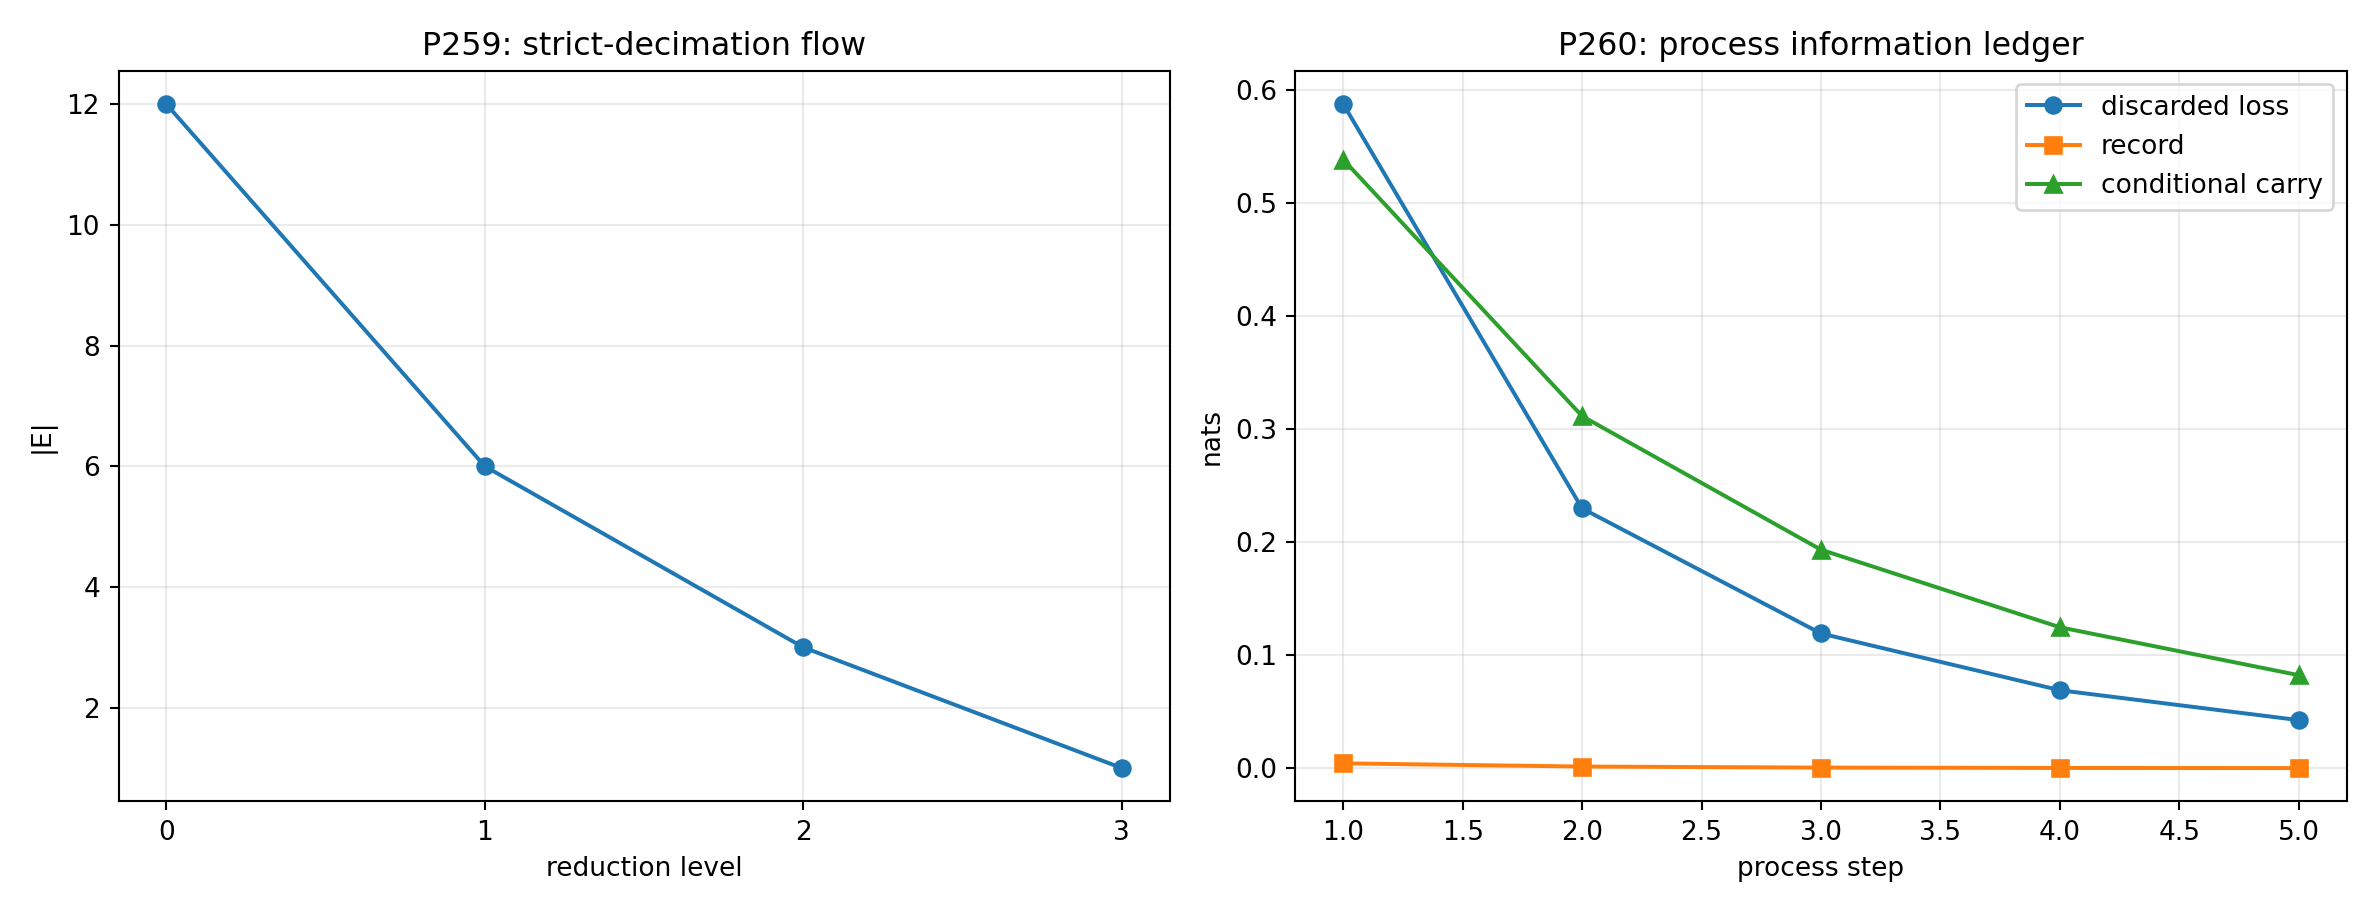
\includegraphics[width=0.97\textwidth]{FIN_Programs_255_266_Figures/p259_p260_rg_information_ledger.png}
\caption{Ściśle malejący przepływ kontekstów i wieloczasowy bilans rozróżnialności.}
\end{figure}

\chapter{9. P260 --- wieloczasowy tensor bilansu informacji}

Niech \(M_k\) będzie wspólnym kanałem dla dwóch hipotez \(p_{k-1},q_{k-1}\):

\[
p_k=M_kp_{k-1},\qquad q_k=M_kq_{k-1}.
\]

Definiujemy stratę kroku:

\[
\ell_k
=
D(p_{k-1}\Vert q_{k-1})
-D(p_k\Vert q_k)
\geq0.
\]

Dla instrumentu zapisującego wynik \(y\) reguła łańcuchowa daje:

\[
D(p_k\Vert q_k)
=
D(r_k^p\Vert r_k^q)
+
\sum_y r_k^p(y)
D(p_k(\cdot|y)\Vert q_k(\cdot|y)).
\]

Stąd nowy obiekt --- \textbf{Process Information Ledger}:

\[
\boxed{
D_{\rm input}
=
\ell_{k,\rm env}
+D_{k,\rm record}
+D_{k,\rm conditional}
}.
\]

W pięciu krokach:

\begin{center}
\begingroup\small
\setlength{\tabcolsep}{2.5pt}
\renewcommand{\arraystretch}{1.16}
\begin{longtable}{@{}p{0.420\textwidth}p{0.420\textwidth}@{}}
\toprule
\textbf{Wielkość} & \textbf{Wynik} \\
\midrule
\endhead
całkowita utrata rozró\.znialności & 1.0483671856 nat \\
suma strat krokowych & 1.0483671856 nat \\
residual teleskopowy & 0 \\
maksymalny residual chain rule & \(6.94\times10^{-17}\) \\
minimalna strata w 1000 dodatkowych parach & 0.0876620 nat \\
\bottomrule
\end{longtable}
\endgroup
\end{center}

Ledger rozdziela to, co traci system, co trafia do rekordu aparatu i co pozostaje w stanie warunkowym. Nie przelicza natów na d\.zule. Do tego potrzeba Hamiltonianu, temperatury, kąpieli i protokołu resetu.

\chapter{10. P261 --- dynamiczny completion defect}

\section{10.1. Zamro\.zona mapa}

Zbadano dokładnie jeden atom:

\[
\mathcal C_{\rm amp}:
K_{\rm legacy}
\longmapsto
\frac{K_{\rm legacy}}{\alpha_{\rm geo}}.
\]

Mapa:

\begin{itemize}
\item 
usuwa wyłącznie amplitudę;

\item 
zachowuje legacy \(\omega=\pi/4\), \(\phi=\pi/6\), \(\beta_{\rm tors}=0.01\);

\item 
stosuje ten sam przepis \(A=\operatorname{diag}(W\mathbf1)-W\);

\item 
nie dodaje znaku, przesunięcia, dodatniości ani kompresji \(d^\eta\).

\end{itemize}

\section{10.2. Wynik}

\begin{center}
\begingroup\small
\setlength{\tabcolsep}{2.5pt}
\renewcommand{\arraystretch}{1.16}
\begin{longtable}{@{}p{0.239\textwidth}p{0.279\textwidth}p{0.342\textwidth}@{}}
\toprule
\textbf{Wielkość} & \textbf{Strict} & \textbf{Legacy po \(\mathcal C_{\rm amp}\)} \\
\midrule
\endhead
\(\lambda_{\min}(A)\) & \(-2.64\times10^{-16}\) & \(-7.7101445443\) \\
\(\lambda_{\min}(A_{HH})\) & 1.1710910206 & \(-5.8247982640\) \\
dodatni biegun resolwenty & brak & \(z=5.8247982640\) \\
\bottomrule
\end{longtable}
\endgroup
\end{center}

Projektowy defect samoenergii:

\begin{center}
\begingroup\small
\setlength{\tabcolsep}{2.5pt}
\renewcommand{\arraystretch}{1.16}
\begin{longtable}{@{}p{0.420\textwidth}p{0.420\textwidth}@{}}
\toprule
\textbf{\(z\)} & \textbf{\(\|\widehat\Sigma_{\rm strict}-\widehat\Sigma_{\rm legacy}\|_F\)} \\
\midrule
\endhead
6.5 & 1.2721 \\
8 & 1.1547 \\
12 & 1.0242 \\
20 & 0.9455 \\
\bottomrule
\end{longtable}
\endgroup
\end{center}

Wniosek:

\[
\boxed{
\mathcal C_{\rm amp}
\text{ nie jest mostem do dodatniej klasy Stieltjesa strict}
}
\]

\textbf{\statusProven{}} dla tej mapy.

Wynik nie obala mostu zawierającego jawny strict-side sign/\allowbreak{}shift, zmianę fazy, częstotliwości, nieliniową kompresję i źródło selektora. Nie rozpoczyna się role transfer.

\begin{figure}[htbp]
\centering
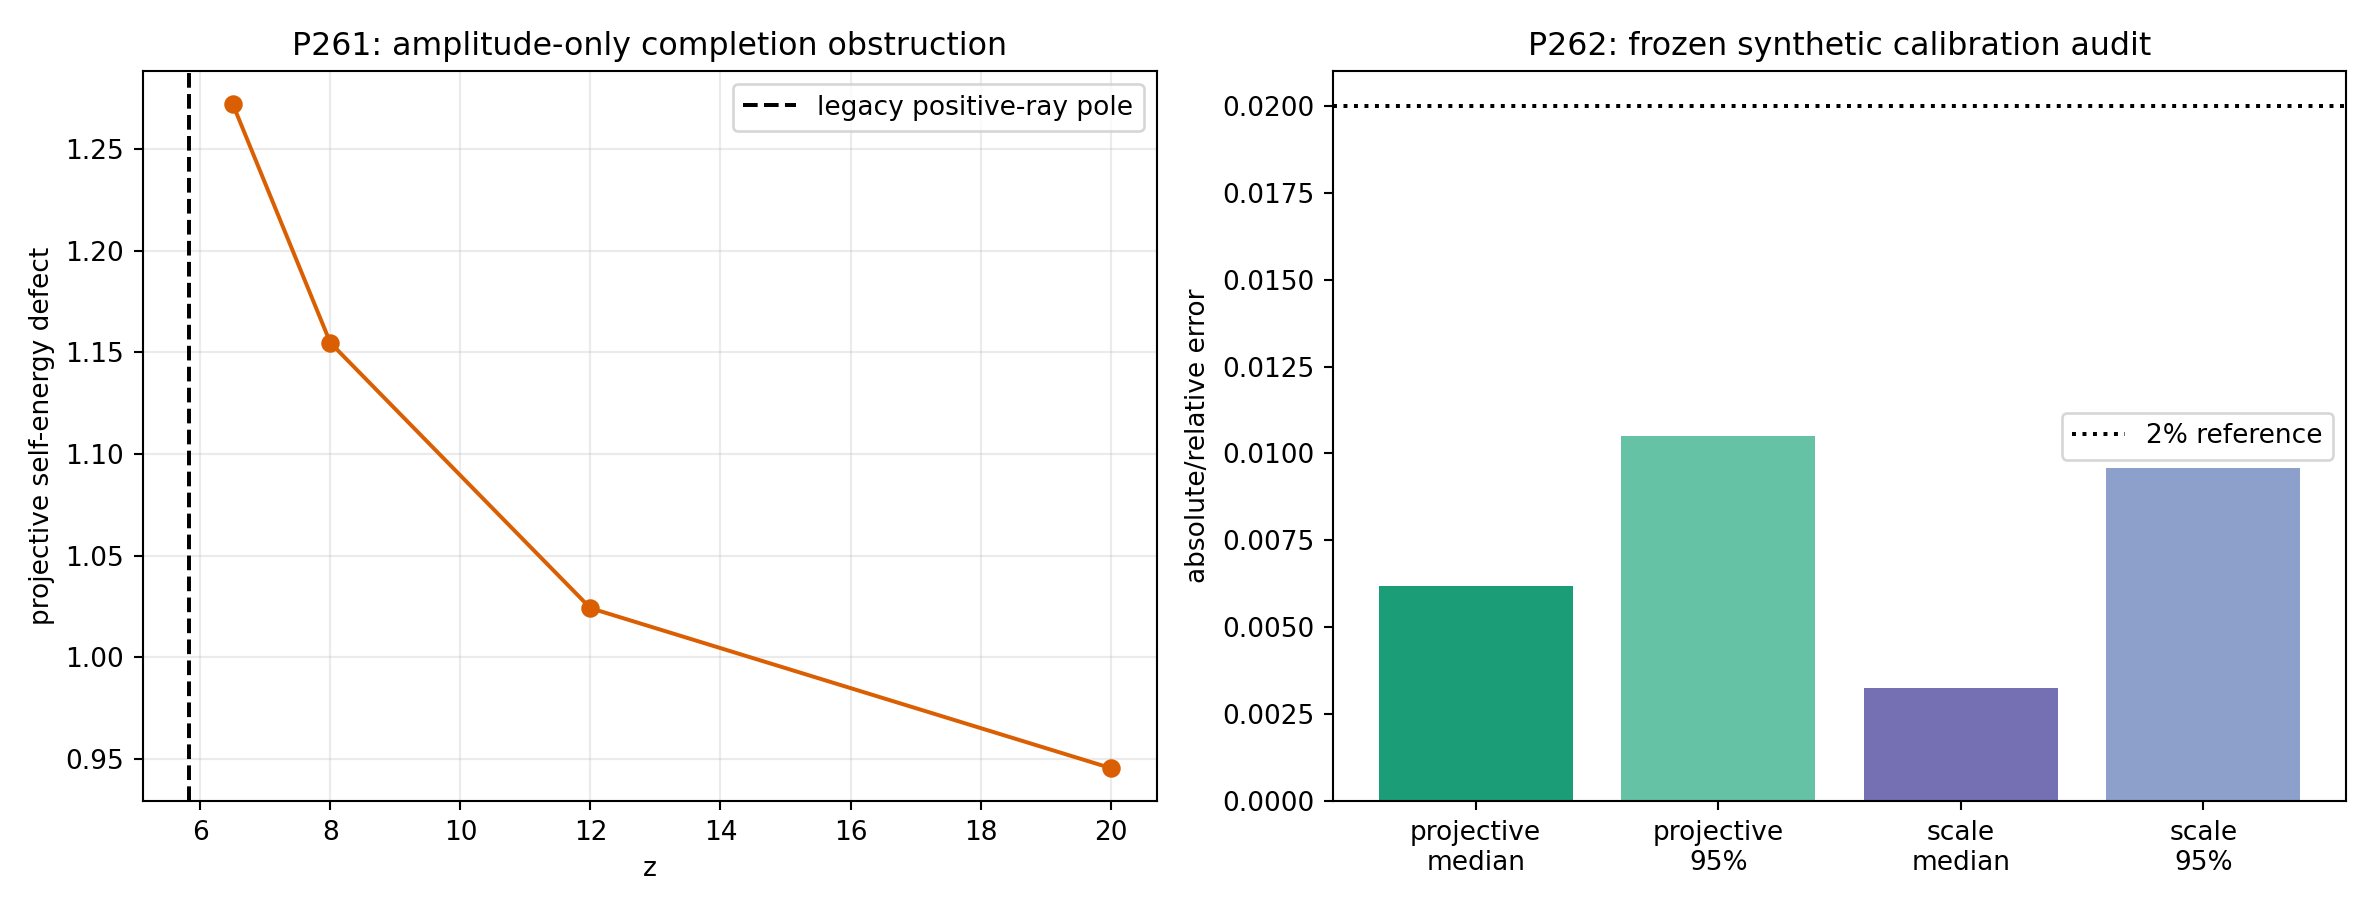
\includegraphics[width=0.97\textwidth]{FIN_Programs_255_266_Figures/p261_p262_bridge_fingerprint.png}
\caption{Obstruction amplitude-only completion oraz syntetyczny audyt fingerprint-first/calibration-second.}
\end{figure}

\chapter{11. P262 --- Calibrated Fingerprint Experiment}

Protokół ma kolejność:

\begin{enumerate}
\item 
zamrozić strict fingerprint;

\item 
zebrać macierz przejścia;

\item 
przetestować ilorazy widmowe bez jednostki;

\item 
dopiero później u\.zyć niezale\.znego zegara do wyboru reprezentanta orbity \((cA,\tau/c)\);

\item 
nie zmieniać modelu po unblindingu.

\end{enumerate}

Audyt syntetyczny:

\begin{center}
\begingroup\small
\setlength{\tabcolsep}{2.5pt}
\renewcommand{\arraystretch}{1.16}
\begin{longtable}{@{}p{0.420\textwidth}p{0.420\textwidth}@{}}
\toprule
\textbf{Wielkość} & \textbf{Wynik} \\
\midrule
\endhead
replikacje & 300 \\
zliczenia na przygotowanie & 50 000 \\
mediana błędu fingerprint & 0.00620 \\
95 percentyl błędu fingerprint & 0.01050 \\
mediana względnego błędu skali & 0.00325 \\
95 percentyl względnego błędu skali & 0.00957 \\
joint pass przy progach 0.03/\allowbreak{}0.02 & 1.000 \\
\bottomrule
\end{longtable}
\endgroup
\end{center}

\textbf{\statusStrong{}} jako planowanie metody.

Nie dostarczono niezale\.znie powierzonych zdarzeń. Walidator P241 nie ma czego przyjąć, więc P242 pozostaje niewykonany.

\chapter{12. P263 --- tomografia prądów i pamięci chiralnej}

\section{12.1. No-go vertex POVM}

Skonstruowano:

\[
\rho_\pm
=
\frac{I}{12}
\pm i\epsilon
\left(
|10\rangle\langle2|
-|2\rangle\langle10|
\right),
\qquad \epsilon=0.04.
\]

Oba stany są dodatnie:

\[
\lambda_{\min}(\rho_\pm)=0.0433333.
\]

Mają identyczne populacje:

\[
\operatorname{diag}\rho_+
=
\operatorname{diag}\rho_-,
\]

ale przeciwne prądy czwartej harmonicznej:

\[
C_4(\rho_+)=-0.0150493,
\qquad
C_4(\rho_-)=+0.0150493.
\]

Zatem vertex POVM jest niewystarczający do tomografii prądu. \textbf{\statusProven{}}

\section{12.2. Brakujący instrument}

Dla \(d=1,\ldots,5\) definiujemy hermitowskie obserwable:

\[
\mathcal J_d
=
i\,d\sum_xW_{x,x+d}
\left(
|x+d\rangle\langle x|
-|x\rangle\langle x+d|
\right).
\]

Wtedy:

\[
C_d(\rho)=\operatorname{Tr}(\rho\mathcal J_d).
\]

Pięć obserwabli ma rangę Grama równą 5 i condition number \(15.17\). Mogą zostać zmierzone przez interferometryczne bazy fazowe, ale nie przez sam odczyt wierzchołków.

\(\Xi_E\) wymaga innego eksperymentu: procesowej tomografii generatora przy dwóch dostarczonych skrętach \(\pm h\). Residual rekonstrukcji centralną ró\.znicą wynosi \(4.94\times10^{-11}\).

\chapter{13. P264 --- atlas false positives}

Zamro\.zono pięć testów:

\begin{enumerate}
\item 
strict fingerprint z tolerancją 0.02;

\item 
dodatniość pamięci Stieltjesa;

\item 
składanie kontekstów;

\item 
scaffold kowariancji inwersyjnej;

\item 
dodatni kanał kontrakcji informacji.

\end{enumerate}

Wyniki:

\begin{center}
\begingroup\fontsize{6.5}{7.8}\selectfont
\setlength{\tabcolsep}{2.5pt}
\renewcommand{\arraystretch}{1.16}
\begin{longtable}{@{}p{0.164\textwidth}p{0.142\textwidth}p{0.116\textwidth}p{0.065\textwidth}p{0.115\textwidth}p{0.142\textwidth}p{0.116\textwidth}@{}}
\toprule
\textbf{Zespół} & \textbf{Fingerprint} & \textbf{Stieltjes} & \textbf{Schur} & \textbf{Chiral scaffold} & \textbf{Information} & \textbf{Wszystkie} \\
\midrule
\endhead
strict target & 1.00 & 1.00 & 1.00 & 1.00 & 1.00 & 1.00 \\
positive circulant & 0.00 & 1.00 & 1.00 & 1.00 & 1.00 & 0.00 \\
positive dense & 0.00 & 1.00 & 1.00 & 0.00 & 1.00 & 0.00 \\
signed circulant & 0.00 & 0.24 & 1.00 & 1.00 & 0.03 & 0.00 \\
strict z perturbacją 5\% & 0.52 & 1.00 & 1.00 & 1.00 & 1.00 & 0.52 \\
\bottomrule
\end{longtable}
\endgroup
\end{center}

\begin{figure}[htbp]
\centering
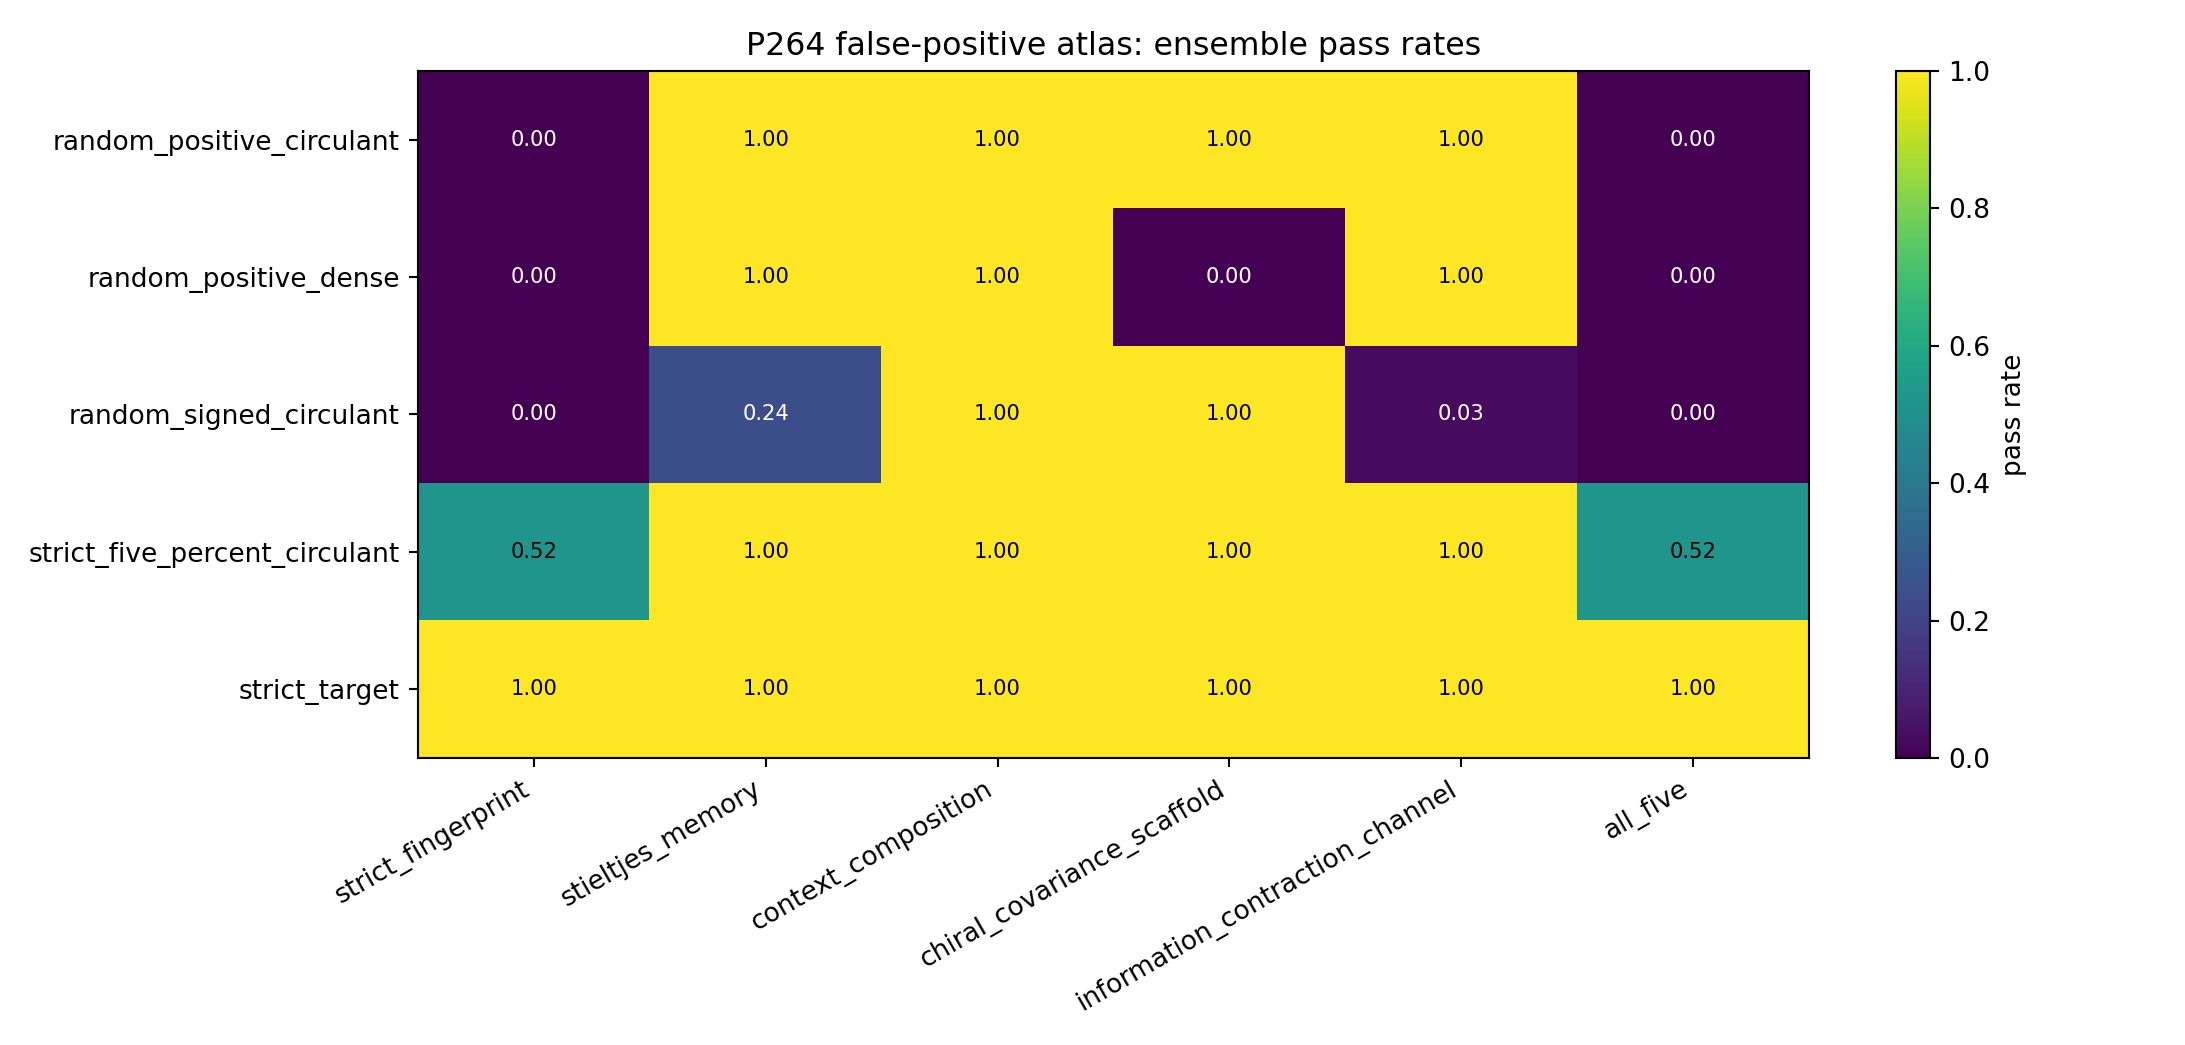
\includegraphics[width=0.97\textwidth]{FIN_Programs_255_266_Figures/p264_false_positive_atlas.png}
\caption{Częstości przejścia pięciu testów w zamrożonych zespołach zerowych.}
\end{figure}

Wniosek:

\begin{itemize}
\item 
twierdzenie Stieltjesa jest silne, ale nie swoiste dla FIN;

\item 
składanie Schura jest uniwersalną algebrą;

\item 
odbiciowa kowariancja jest wspólna dla cyrkulantów;

\item 
największą swoistość ma pełny fingerprint strict;

\item 
5\% perturbacja przechodzi tylko w 52\% prób przy progu 0.02.

\end{itemize}

Nie wolno przedstawiać własności ogólnych dodatniego Laplasjanu jako identyfikatora FIN.

\chapter{14. P265 --- identyfikowalność Adaptive Memory Geometry}

\section{14.1. Dokładny no-go skali}

\[
\exp[-t(cA)]
=
\exp[-(ct)A].
\]

Bez niezale\.znego zegara nie istnieje test odró\.zniający zmianę skali generatora od zmiany czasu. Residual wynosi dokładnie zero.

\section{14.2. Iloraz mechanizmów}

Definiujemy \textbf{Mechanism Identifiability Quotient}:

\[
\mathfrak Q_{\rm id}
=
\frac{
\{\text{generator, zegar, aparat, pamięć, prawo uczenia}\}
}{
\text{równość wszystkich dopuszczonych rekordów operacyjnych}
}.
\]

Tabela syntetyczna:

\begin{center}
\begingroup\small
\setlength{\tabcolsep}{2.5pt}
\renewcommand{\arraystretch}{1.16}
\begin{longtable}{@{}p{0.248\textwidth}p{0.233\textwidth}p{0.160\textwidth}p{0.219\textwidth}@{}}
\toprule
\textbf{Scenariusz} & \textbf{Drift fingerprint} & \textbf{Defect semigrupy} & \textbf{Wymagany dodatkowy zasób} \\
\midrule
\endhead
operator statyczny & 0 & 0 & brak \\
skala generatora albo zegara & \(8.88\times10^{-16}\) & 0 & niezale\.zny zegar \\
niejednorodna zmiana generatora & 0.09239 & 0 & fingerprint \\
pamięć aparatu & 0 & 0.09057 & dane wieloczasowe \\
\bottomrule
\end{longtable}
\endgroup
\end{center}

Migawki \(A_0,A_1,\ldots,A_r\) nie identyfikują unikalnego pola wektorowego \(\dot A=F(A,\mathcal R)\). Nieskończenie wiele funkcji \(F\) interpoluje skończoną trajektorię. Potrzebne są interwencje, rekord aparatu i hold-out.

\chapter{15. P266 --- benchmark biologiczno-cybernetyczny}

FIN porównano z:

\begin{itemize}
\item 
60 rezerwuarami o identycznym widmie i losowej orientacji;

\item 
60 losowymi rezerwuarami symetrycznymi o tej samej liczbie stanów i promieniu spektralnym.

\end{itemize}

Ka\.zdy model miał:

\begin{itemize}
\item 
12 stanów;

\item 
ten sam ciąg wejściowy;

\item 
liniowy readout;

\item 
identyczną procedurę train/\allowbreak{}test;

\item 
zadanie odtworzenia opóźnień 1--20.

\end{itemize}

\begin{center}
\begingroup\small
\setlength{\tabcolsep}{2.5pt}
\renewcommand{\arraystretch}{1.16}
\begin{longtable}{@{}p{0.415\textwidth}p{0.169\textwidth}p{0.277\textwidth}@{}}
\toprule
\textbf{Metryka FIN} & \textbf{Wartość} & \textbf{Percentyl wśród 120 kontroli} \\
\midrule
\endhead
linear memory capacity 1--20 & 4.0601 & 0.000 \\
efektywny wymiar controllability & 1.0698 & 0.0417 \\
kroki powrotu do \(10^{-3}\) & 135 & 1.000 \\
minimalny readout dla 95\% Grama & 1 & 0.0917 \\
\bottomrule
\end{longtable}
\endgroup
\end{center}

\begin{figure}[htbp]
\centering
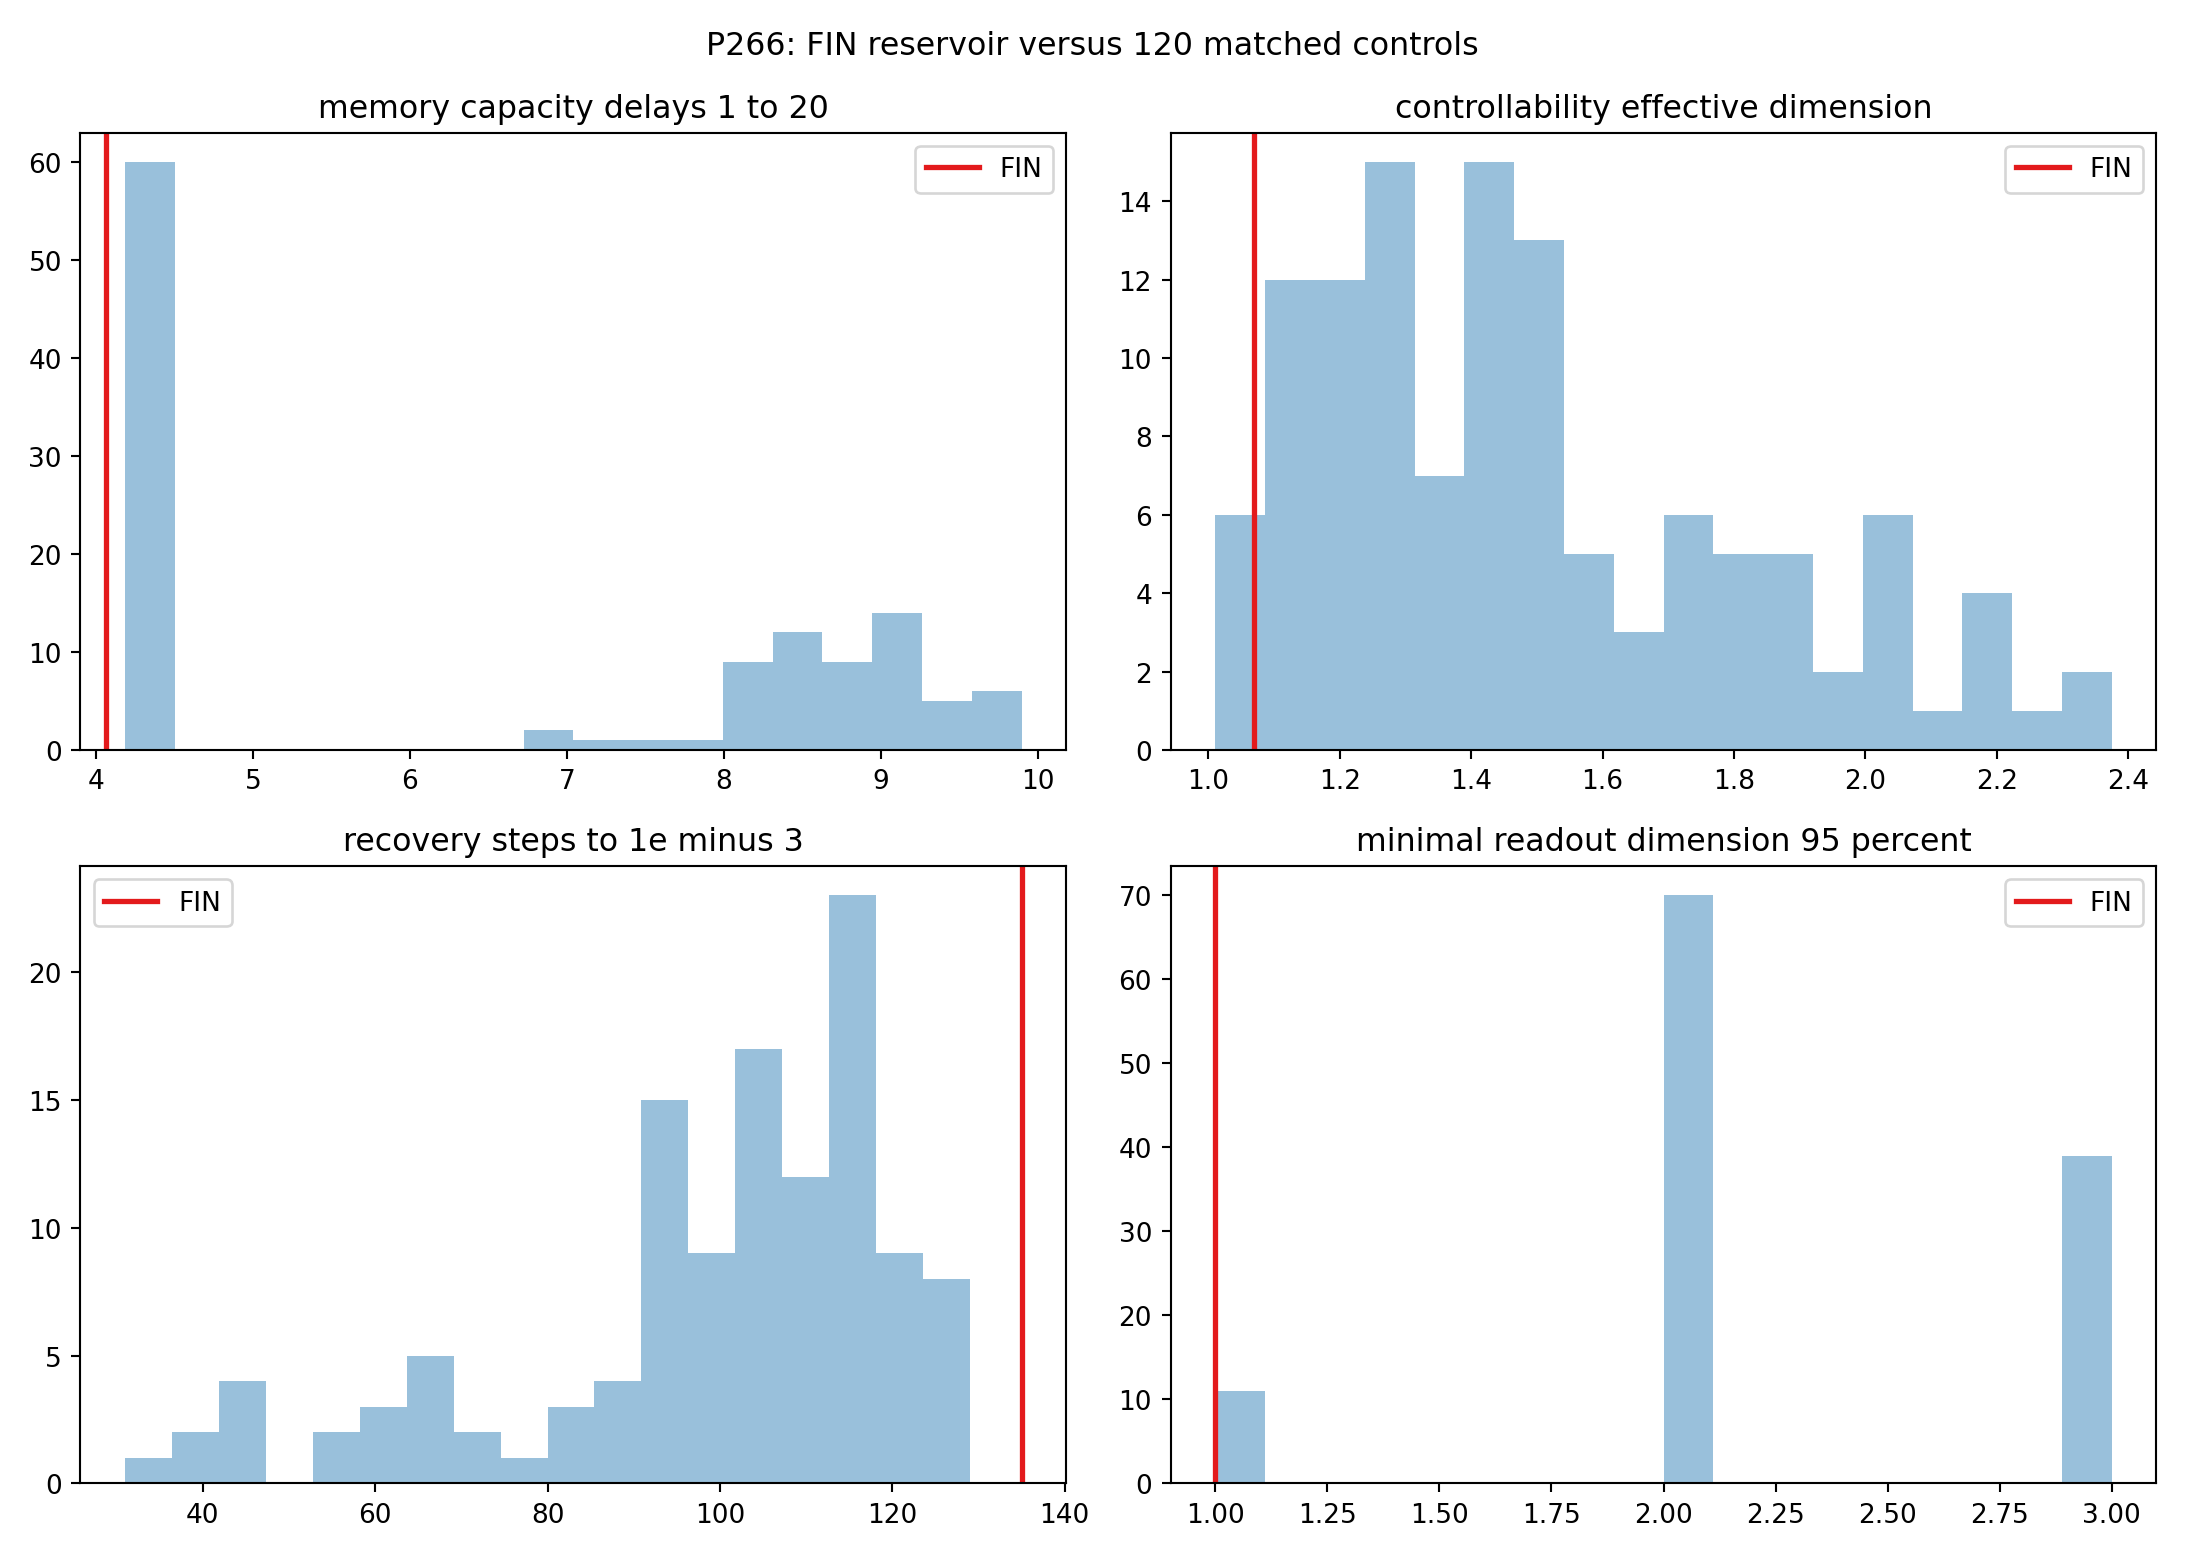
\includegraphics[width=0.97\textwidth]{FIN_Programs_255_266_Figures/p266_reservoir_benchmark.png}
\caption{Rezerwuar FIN na tle 120 kontroli dopasowanych wymiarem lub widmem.}
\end{figure}

FIN jest outlierem, ale nie w kierunku przewagi:

\begin{itemize}
\item 
ma najni\.zszą pojemność pamięci w badanym zestawie;

\item 
ma najwolniejszy powrót dla zadanego zaburzenia;

\item 
jego dostępna dynamika wejście--wyjście jest bliska jednowymiarowej.

\end{itemize}

\textbf{\statusRefuted{}} jako hipoteza o automatycznej przewadze nad standardowym rezerwuarem 12-stanowym w tym benchmarku.

Nie jest obalona mo\.zliwość, \.ze inny input, nieliniowy readout albo jawne prawo adaptacji zmieni wynik. Taki wariant musi jednak pokonać kontrole na danych hold-out.

\chapter{16. Nowe obiekty teoretyczne O16--O25}

\begin{center}
\begingroup\fontsize{7}{8.4}\selectfont
\setlength{\tabcolsep}{2.5pt}
\renewcommand{\arraystretch}{1.16}
\begin{longtable}{@{}p{0.055\textwidth}p{0.206\textwidth}p{0.305\textwidth}p{0.067\textwidth}p{0.228\textwidth}@{}}
\toprule
\textbf{ID} & \textbf{Obiekt} & \textbf{Definicja} & \textbf{Status} & \textbf{Co rozwiązuje} \\
\midrule
\endhead
O16 & Positive Operator Memory Measure & \(\mathsf M_E=\sum_\mu BP_\mu B^\ast\delta_\mu\) & \statusProven{} & klasyfikuje dokładną pamięć \\
O17 & Minimal Hidden Realization Quotient & \((C,B)/{\sim_\Sigma}\) & \statusProven{} & oddziela widzialne środowisko od niewidzialnych trybów \\
O18 & Schur Context Category & \(E\mapsto\operatorname{Schur}_{V\setminus E}(zI+A)\) & \statusProven{} & typuje poprawne redukcje \\
O19 & Chiral Memory Kubo Tensor & \(\Xi=B'RB^\ast+BRB'^\ast-BRC'RB^\ast\) & \statusProven{} & łączy flux response z pamięcią \\
O20 & Size-Restoration Obstruction & brak \(\mathcal E_n\) między ró\.znymi rozmiarami & \statusProven{} & wyjaśnia, dlaczego naiwny fixed point jest źle typowany \\
O21 & Process Information Ledger & \(\ell_{\rm env}+D_{\rm record}+D_{\rm cond}\) & \statusProven{} & rozdziela utratę i zapis \\
O22 & Amplitude Completion Obstruction & dodatni biegun i ujemne widmo po \(\mathcal C_{\rm amp}\) & \statusProven{} & zamyka jeden atom mostu \\
O23 & Current Tomography Instrument & \(\{\mathcal J_d\}_{d=1}^5\) + twist process tomography & \statusProven{}/\allowbreak{}\statusStrong{} & domyka brak vertex POVM dla prądów \\
O24 & Mechanism Identifiability Quotient & mechanizmy modulo równość rekordów & \statusProven{} & oddziela zegar, skalę, pamięć i drift \\
O25 & Matched Reservoir Null Benchmark & FIN kontra kontrole o tym samym \(N,\rho\) i protokole & \statusStrong{} & chroni analogie biologiczne przed nadinterpretacją \\
\bottomrule
\end{longtable}
\endgroup
\end{center}

Najwa\.zniejszym nowym obiektem jest O17. Pokazuje, \.ze "środowisko" odzyskane z pamięci jest klasą minimalnych realizacji, a nie unikalnym światem mikroskopowym.

\chapter{17. Próby falsyfikacji}

\begin{center}
\begingroup\small
\setlength{\tabcolsep}{2.5pt}
\renewcommand{\arraystretch}{1.16}
\begin{longtable}{@{}p{0.270\textwidth}p{0.362\textwidth}p{0.228\textwidth}@{}}
\toprule
\textbf{Teza} & \textbf{Próba zniszczenia} & \textbf{Wynik} \\
\midrule
\endhead
ka\.zda \(\Sigma_E\) jest Stieltjesa & wszystkie 4094 konteksty, pochodne do rzędu 4 & przetrwała \\
ukryty sektor jest unikalny & dodano dwa rozsprzę\.zone tryby & obalona \\
diagram kontekstów jest funktorem & 20 000 zagnie\.zd\.zonych redukcji & przetrwała \\
\(\Xi\) jest ad hoc & wyprowadzono jako pochodną resolwenty & obalona krytyka ad hoc \\
\(\Xi\) wybiera orientację & inwersja daje parę \(\pm\Xi\) & teza obalona \\
naiwny decimation RG ma fixed point & wymiar \(12>6>3>1\) & teza źle typowana \\
information loss jest energią & brak skali, kąpieli i Hamiltonianu & teza obalona \\
sama amplituda łączy legacy i strict & ujemne widmo i dodatni biegun & teza obalona \\
vertex POVM mierzy prąd & \(\rho,\rho^\ast\) o tych samych populacjach & teza obalona \\
Stieltjes/\allowbreak{}Schur identyfikuje FIN & dodatnie losowe Laplasjany przechodzą & teza obalona \\
jeden czas rozdziela zegar i generator & \(\exp[-tcA]=\exp[-ctA]\) & niemo\.zliwe \\
FIN ma naturalną przewagę reservoir & 120 matched controls & teza obalona w zadanym benchmarku \\
\bottomrule
\end{longtable}
\endgroup
\end{center}

\chapter{18. Relacja do istniejącej matematyki}

\section{18.1. Mori--Zwanzig i eliminacja stopni swobody}

Pamięć po projekcji nie jest nową ideą. O16--O19 umieszczają FIN w skończonym, dokładnym odpowiedniku formalizmu projekcyjnego. Ró\.znicą jest jawna, operatorowo-Stieltjesowska klasyfikacja wszystkich kontekstów konkretnego generatora strict.

\section{18.2. Realization theory}

O17 jest standardowym typem wyniku teorii realizacji: dane wejście--wyjście identyfikują minimalną realizację do równowa\.zności, nie dowolne stany nieobserwowalne. Nowość dla FIN polega na znalezieniu konkretnego niewidzialnego trybu i na wpisaniu nieidentyfikowalności do granic ontologicznych.

\section{18.3. Process tensors}

Proces tensorowy uczy, \.ze wieloczasowy proces jest określony przez odpowiedzi na sekwencje interwencji, a nie przez jedną mapę stanu. O21 i O24 są klasycznym, skończonym rdzeniem tej samej dyscypliny. Nie są jeszcze kwantowym process tensorem FIN.

\section{18.4. Reservoir computing}

Memory capacity jest ograniczona wymiarem rezerwuaru, ale szczegółowa pojemność zale\.zy od widma, controllability i readoutu. P266 pokazuje, \.ze regularność FIN nie gwarantuje przewagi. To kontrolowana analogia, nie identyfikacja z mózgiem.

\chapter{19. Rekomendowane programy 267--280}

\section{P267 --- Uniqueness of the operator memory measure}

Udowodnić jednoznaczność atomowej miary \(\mathsf M_E\) z funkcji \(\Sigma_E(z)\) oraz stabilność odzyskiwania biegunów przy szumie.

\textbf{Prawdopodobieństwo:} 0.92.\\
\textbf{Stop rule:} nie interpretować biegunów niewidzialnych.

\section{P268 --- Formalny core kategorii Schura}

Zapisać O18 w Lean/\allowbreak{}Mathlib, Coq albo Isabelle: obiekty, morfizmy, identyczność, łączność i dodatniość.

\textbf{Prawdopodobieństwo:} 0.80.

\section{P269 --- Minimalność instrumentu prądowego}

Udowodnić minimalną liczbę ustawień POVM potrzebnych do odzyskania pięciu \(C_d\), uwzględniając straty, dark counts i nieznane fazy.

\textbf{Prawdopodobieństwo:} 0.85.

\section{P270 --- Size-restoring RG equivalence}

Skonstruować jedną jawną mapę \(\mathcal E_n\), która porównuje ró\.zne rozmiary bez dopasowywania do strict target, albo udowodnić no-go dla lokalnych, circulant-preserving embeddings.

\textbf{Prawdopodobieństwo konstrukcji:} 0.35.\\
\textbf{Prawdopodobieństwo no-go:} 0.75.

\section{P271 --- Quantum Process Information Ledger}

Zastąpić kanały klasyczne instrumentami CP i udowodnić bilans O21 dla relative entropy procesów z pamięcią.

\textbf{Prawdopodobieństwo:} 0.62.

\section{P272 --- Następny pojedynczy atom completion}

Po no-go amplitude-only dopuścić dokładnie jeden jawny strict-side atom: globalny sign/\allowbreak{}positive shift \textbf{albo} nonlinear damping completion. Mapa i progi muszą być zamro\.zone przed porównaniem z strict.

\textbf{Prawdopodobieństwo bridge:} 0.25.\\
\textbf{Prawdopodobieństwo wartościowego obstruction:} 0.80.

\section{P273 --- External calibrated fingerprint}

Pozyskać pakiet P241 z niezale\.znym providerem, registrarem i analystą. Najpierw fingerprint, potem kalibracja, jedna tura P242.

\textbf{Prawdopodobieństwo metodologiczne:} 0.75.\\
\textbf{Prawdopodobieństwo wykonania bez partnera laboratoryjnego:} niskie.

\section{P274 --- Chiral two-flux process tomography}

Zaprojektować aparaturę realizującą \(\pm h\), zmierzyć \(\mathcal J_d\) oraz zrekonstruować \(\Xi_E(z)\) z niepewnością.

\textbf{Prawdopodobieństwo wykonalności do oceny przez fizyka:} 0.60.

\section{P275 --- Analityczne false-positive bounds}

Wyprowadzić prawdopodobieństwo przejścia strict fingerprint dla zamro\.zonych zespołów random Laplacian zamiast polegać tylko na Monte Carlo.

\textbf{Prawdopodobieństwo:} 0.72.

\section{P276 --- Two-clock/\allowbreak{}two-time identifiability theorem}

Określić minimalny zestaw dwóch czasów, niezale\.znego zegara i kontroli, który oddziela uniform scaling, shape drift i memory defect.

\textbf{Prawdopodobieństwo:} 0.90.

\section{P277 --- Causal identification of the adaptive law}

Zamrozić skończoną rodzinę praw \(F(A,\mathcal R)\), projekt interwencji i hold-out. Nie dopuszczać dowolnego universal approximator.

\textbf{Prawdopodobieństwo rozstrzygnięcia:} 0.65.

\section{P278 --- Nonlinear matched reservoir benchmark}

Powtórzyć P266 dla NARMA, parity, channel equalization i prediction tasks z jednakowym bud\.zetem parametrów oraz prerejestrowanym rankingiem.

\textbf{Prawdopodobieństwo:} 0.80.

\section{P279 --- Conditional thermodynamic bridge}

Po dostarczeniu \((H,T,\text{bath},\text{reset protocol})\) zbadać, kiedy O21 staje się bilansem pracy/\allowbreak{}produkcji entropii. Wynik musi być jawnie conditioned-on-CA, nie strict.

\textbf{Prawdopodobieństwo matematyczne:} 0.75.\\
\textbf{Prawdopodobieństwo strict source:} niskie.

\section{P280 --- Two-torsor operational section}

Połączyć niezale\.zny clock/\allowbreak{}scale section z dostarczonym orientation resource w jednym protokole, bez twierdzenia, \.ze jeden zasób generuje drugi.

\textbf{Prawdopodobieństwo konstrukcji warunkowej:} 0.85.\\
\textbf{Strict selector closure:} nie jest celem programu.

\chapter{20. Ranking następnej rundy}

\begin{center}
\begingroup\small
\setlength{\tabcolsep}{2.5pt}
\renewcommand{\arraystretch}{1.16}
\begin{longtable}{@{}p{0.183\textwidth}p{0.257\textwidth}p{0.420\textwidth}@{}}
\toprule
\textbf{Ranga} & \textbf{Program} & \textbf{Powód} \\
\midrule
\endhead
1 & P267 & domyka matematyczną identyfikowalność pamięci \\
2 & P269 & zamienia no-go vertex POVM w minimalny instrument \\
3 & P276 & najkrótszy most od ilorazu skali do poprawnego eksperymentu \\
4 & P268 & formalizuje centralną kategorię \\
5 & P275 & mierzy rzeczywistą swoistość FIN \\
6 & P271 & rozszerza ledger do procesów kwantowych \\
7 & P277 & rozstrzyga, czy adaptacja jest identyfikowalna \\
8 & P278 & kontynuuje falsyfikację analogii neuronowej \\
9 & P270 & wysoka nagroda, lecz brak size-restoring map \\
10 & P272 & tylko jeden nowy atom bridge \\
11 & P274 & wymaga oceny i aparatury laboratoryjnej \\
12 & P273 & wymaga rzeczywiście niezale\.znych danych \\
13 & P279 & tylko jako teoria warunkowa \\
14 & P280 & domyka operacyjny pakiet, nie strict selector \\
\bottomrule
\end{longtable}
\endgroup
\end{center}

\chapter{21. Granice zgodne z guardrails}

Runda 255--266 nie eksportuje:

\begin{itemize}
\item 
niepremisowego selektora;

\item 
rozładowania QW-2191;

\item 
kanonicznej jednostki czasu, długości, masy, energii lub działania;

\item 
pełnej mapy legacy->strict;

\item 
role transfer dla legacy;

\item 
źródła \(\beta,\eta,\omega,\phi\) strict;

\item 
unikalnego środowiska mikroskopowego;

\item 
unikalnego prawa adaptacji;

\item 
fizycznego aparatu lub laboratoryjnego rekordu;

\item 
\(L_{\rm total}\), Modelu Standardowego, GR ani ToE.

\end{itemize}

P261 zamyka wyłącznie amplitude-only completion. Kolejny program mostowy jest dopuszczalny tylko dla jednego nowego, jawnie typowanego atomu.

\chapter{22. Werdykt końcowy}

Najgłębszy wynik tej rundy nie polega na znalezieniu nowej stałej fizycznej. Polega na zmianie statusu słowa "pamięć".

\[
\boxed{
\begin{gathered}
\text{Pamięć FIN jest dodatnią miarą operatorową widzianą przez kontekst,}\\
\text{a nie unikalnym ukrytym światem.}
\end{gathered}
}
\]

Samoenergia określa minimalną klasę realizacji wejście--wyjście. Redukcje tych klas składają się kategoryjnie, chiralny skręt ma dobrze określony tangent, a informacja posiada dokładny ledger operacyjny. Jednocześnie skala zegara, źródło orientacji, mikroskopowa realizacja i prawo adaptacji pozostają nieidentyfikowalne bez dodatkowych operacji.

To wzmacnia FIN jako skończoną teorię operatorową pamięci i procesu. Nie przekształca jej jeszcze w teorię fizyczną.

\chapter{23. Wybrane źródła porównawcze}

\begin{enumerate}
\item 
S. Belyi, E. Tsekanovskii, \emph{Stieltjes like functions and inverse problems for systems with Schrödinger operator}, \href{https://arxiv.org/abs/0708.0452}{arXiv:0708.0452}.

\item 
Y. T. Lin, Y. Tian, M. Anghel, D. Livescu, \emph{Data-driven learning for the Mori--Zwanzig formalism}, \href{https://arxiv.org/abs/2101.05873}{arXiv:2101.05873}.

\item 
F. A. Pollock et al., \emph{Operational Markov condition for quantum processes}, \href{https://arxiv.org/abs/1801.09811}{arXiv:1801.09811}.

\item 
H. Jaeger, \emph{Short term memory in echo state networks}, GMD Report 152, \href{https://publica.fraunhofer.de/entities/publication/9dfaead1-4dc0-4e3c-b89b-596f50f671c1}{Fraunhofer record and DOI}.

\item 
F. Dörfler, F. Bullo, \emph{Kron Reduction of Graphs with Applications to Electrical Networks}, \href{https://arxiv.org/abs/1102.2950}{arXiv:1102.2950}.

\end{enumerate}

Źródła słu\.zą do klasyfikacji istniejącej matematyki. Nie są dowodem fizycznej równowa\.zności FIN z \.zadnym z tych formalizmów.

\chapter{24. Reprodukcja}

``bash MPLCONFIGDIR=/\allowbreak{}tmp/\allowbreak{}matplotlib-p255-266 \\
python3 fin\_programs\_255\_266.py

MPLCONFIGDIR=/\allowbreak{}tmp/\allowbreak{}matplotlib-p255-266 \\
python3 -m unittest -v test\_fin\_programs\_255\_266.py ``

Oczekiwany wynik:

\begin{itemize}
\item 
4094 konteksty P255;

\item 
20 000 łańcuchów P257;

\item 
300 replikacji P262;

\item 
401 wierszy atlasu P264;

\item 
121 rezerwuarów P266;

\item 
15/\allowbreak{}15 testów.

\end{itemize}


\clearpage
\chapter*{Certyfikat reprodukcji}
\addcontentsline{toc}{chapter}{Certyfikat reprodukcji}
\begin{Verbatim}[fontsize=\small]
MPLCONFIGDIR=/tmp/matplotlib-p255-266 \
python3 fin_programs_255_266.py

MPLCONFIGDIR=/tmp/matplotlib-p255-266 \
python3 -m unittest -v test_fin_programs_255_266.py
\end{Verbatim}
Oczekiwany wynik testów: 15 passed, 0 failed.  Dane P262, P264, P265 i P266
są syntetyczne; nie są rekordem laboratoryjnym.
\end{document}
